\documentclass[14pt, aspectratio=169, handout]{beamer}
\usetheme{Copenhagen}
\usecolortheme{seahorse}
\setbeamertemplate{navigation symbols}{}
\setbeamertemplate{headline}{}

%\usepackage{pgfpages}
%\pgfpagesuselayout{4 on 1}[a4paper, border shrink=5mm]

\usepackage{graphicx} % Required for inserting images
\usepackage{multicol}
%\usepackage{enumitem}
\usepackage{amsfonts}
\usepackage{amsmath}
\usepackage{xcolor}
\definecolor{myblue}{RGB}{0, 0, 255} 
\definecolor{mygreen}{RGB}{0, 180, 80}
\definecolor{myred}{RGB}{153, 0, 0}
\definecolor{myorange}{RGB}{255, 153, 51}
\definecolor{mypurple}{RGB}{102, 0, 204}
\usepackage{tikz}

%--- commands for transform arrows----------------
\newcommand{\transform}[2]{%
    \begin{tikzpicture}
        % Open circle
        \draw[thick] (0,0) circle (0.1);
        % Line with number above and adjustable length
        \draw[thick] (0.1,0) -- (#2,0) node[midway, above] {#1};
        % Filled circle
        \filldraw[thick] (#2,0) circle (0.1);
    \end{tikzpicture}%
}
\newcommand{\invtransform}[2]{%
    \begin{tikzpicture}
        % filled circle
        \filldraw[thick] (0,0) circle (0.1);
        % Line with number above and adjustable length
        \draw[thick] (0.1,0) -- (#2 -0.1,0) node[midway, above] {#1};
        % open circle
        \draw[thick] (#2,0) circle (0.1);
    \end{tikzpicture}%
}
\newcommand{\verticaltransform}[4]{%
    \begin{tikzpicture}
        % Open circle at the bottom with text below
        \filldraw[thick] (0,0) circle (0.1) node[below=3pt] {$#4$};
        % Vertical line with number on the left
        \draw[thick] (0,0.1) -- (0,#2 -0.1) node[midway, left] {#1};
        % Filled circle at the top with text above
        \draw[thick] (0,#2) circle (0.1) node[above=3pt] {$#3$};
    \end{tikzpicture}%
}
\newcommand{\verticalinvtransform}[4]{%
    \begin{tikzpicture}
        % Open circle at the bottom with text below
        \draw[thick] (0,0) circle (0.1) node[below=3pt] {$#4$};
        % Vertical line with number on the left
        \draw[thick] (0,0.1) -- (0,#2) node[midway, left] {#1};
        % Filled circle at the top with text above
        \filldraw[thick] (0,#2) circle (0.1) node[above=3pt] {$#3$};
    \end{tikzpicture}%
}

\definecolor{darkblue}{RGB}{0, 0, 139}
\definecolor{lightblue}{RGB}{173, 216, 230}

\title{SST1 Übungsstunde 8}
\author{Matteo Dietz}
\date{November 2024}

\begin{document}

\maketitle

\begin{frame}{Themenüberblick}
    \begin{itemize}
        \item \textbf{Abtasttheorem}:
        \item[] Digitale Systeme
        \item[] Abgetastete Systeme im Frequenzbereich
        \item[] Aliasing, Interpolation, Kritische Abtastung
        \item[] Interpretation als Entwicklung in ein Orthonormalsystem
    \end{itemize}
\end{frame}


\begin{frame}{Aufgaben für diese Woche}
    \begin{itemize}
        \item[] \textbf{78}, \textbf{79}, \textbf{80}, 81, \textbf{82}, 83, 84, \textbf{85}, 86, \textbf{87}, 88, \textbf{89}, \textbf{90}, 91, \textbf{92}, \textbf{93}, \textbf{94}, 95, \textbf{96}
        \item[] 
        \item[] Die \textbf{fettgedruckten} Übungen empfehle ich, weil sie wesentlich zu eurem Verständnis der Theorie beitragen und/oder sehr prüfungsrelevant sind.
    \end{itemize}
\end{frame}

\begin{frame}{Digitale Systeme}
    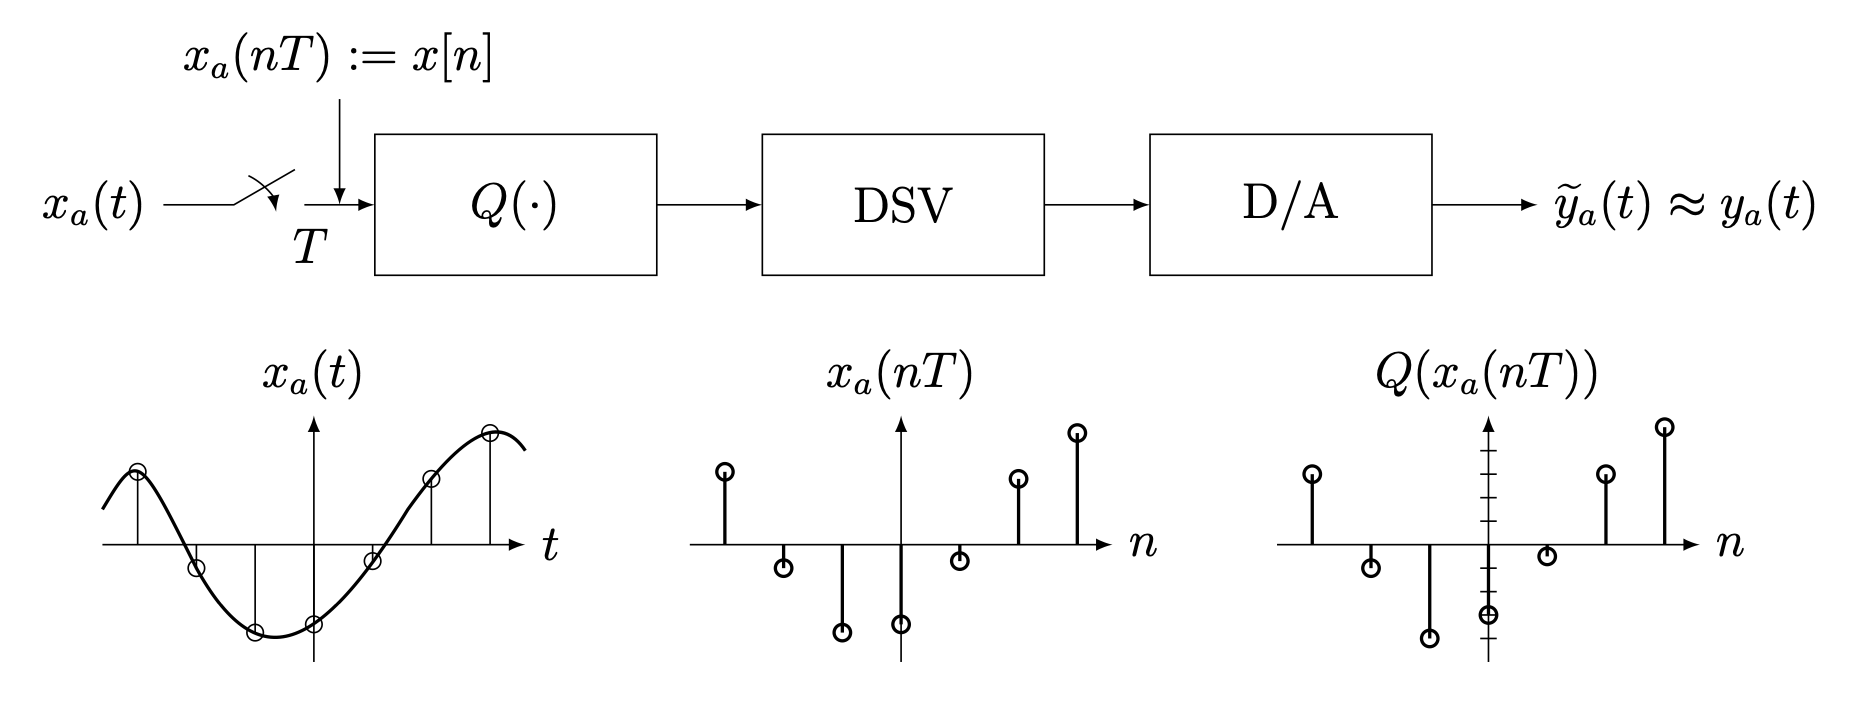
\includegraphics[width=\linewidth]{figures/digitale_sys1.png}
\end{frame}

\begin{frame}{Abgetastete Signale im Frequenzbereich}
    \begin{enumerate}
    \item[1.] Abtastung wird modelliert als Multiplikation mit einem Deltakamm:
    \vspace*{-0.5cm}
    \begin{align*}
        x_{abg.}(t) &= x(t)\delta_T(t) = x(t)\sum_{k=-\infty}^{\infty} \delta(t-kT) \\
        &= \sum_{k=-\infty}^{\infty}x(t)\delta(t-kT) = \sum_{k=-\infty}^{\infty} x(kT)\delta(t-kT)
    \end{align*}
    \vspace*{-0.5cm}
    \item[] \begin{center}
        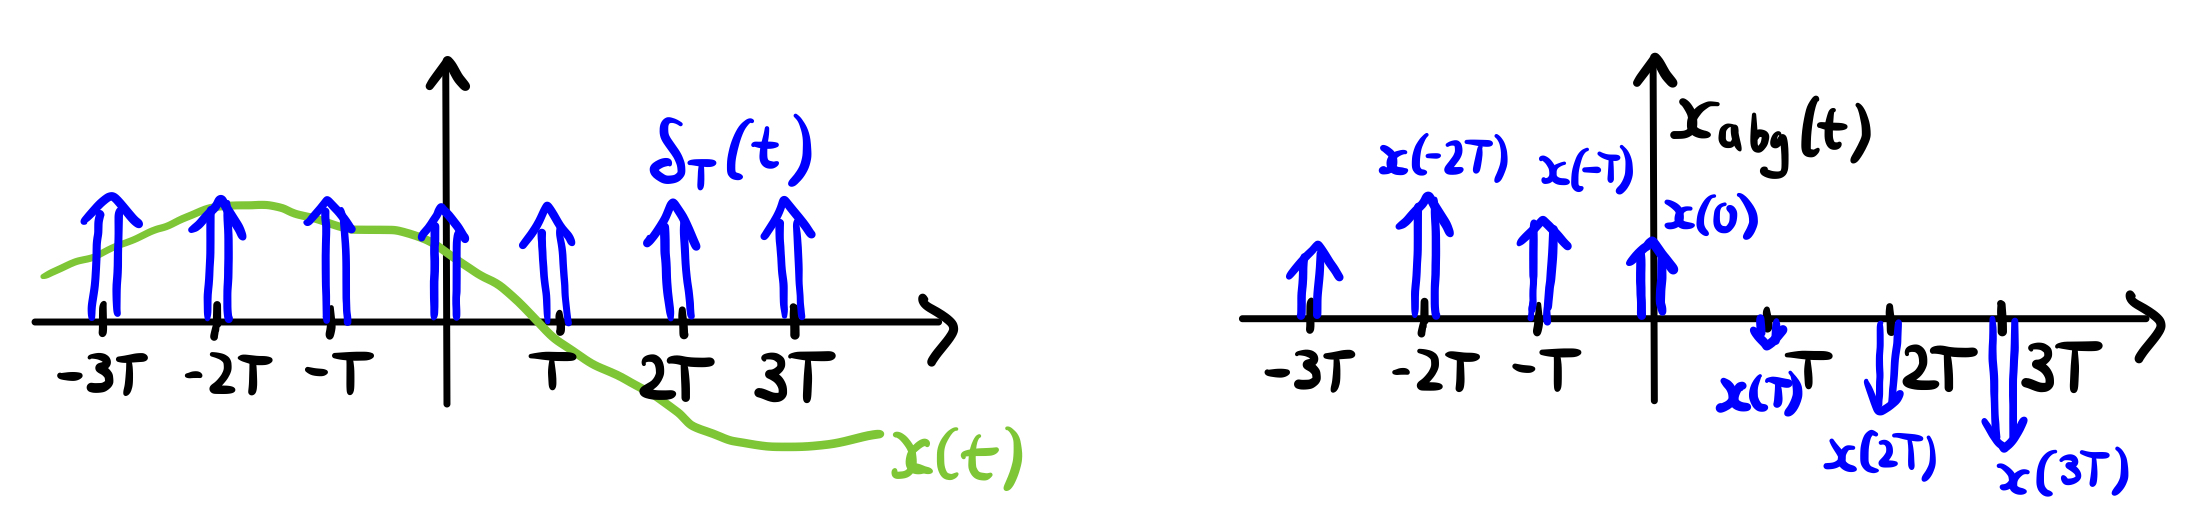
\includegraphics[width=0.8\linewidth]{figures/abtastung1.jpg}
    \end{center}
    \end{enumerate}
\end{frame}

\begin{frame}{Abgetastete Signale im Frequenzbereich}
    \begin{enumerate}
        \item[2.] Wir fouriertransformieren das abgetastete Signal $x_{abg}(t)$.
    \begin{align*}
        \hat{x}_{abg.}(f) &= \mathcal{F}\{x \cdot \delta_T\}(f) = \left( \hat{x} \ast \hat{\delta}_T \right)(f) \\
        &\overset{20.}{=} \left( \hat{x} \ast \frac{1}{T} \sum_{k=-\infty}^\infty \delta\left(\cdot - \frac{k}{T}\right) \right)(f) \\
        &= \frac{1}{T} \sum_{k=-\infty}^\infty \left( \hat{x} \ast \delta \left( \cdot - \frac{k}{T} \right) \right)(f) \\
        &= \frac{1}{T} \sum_{k = -\infty}^\infty \hat{x}\left( f- \frac{k}{T} \right)
    \end{align*}
    \end{enumerate}
\end{frame}

\begin{frame}{Abgetastete Signale im Frequenzbereich}
    \begin{center}
        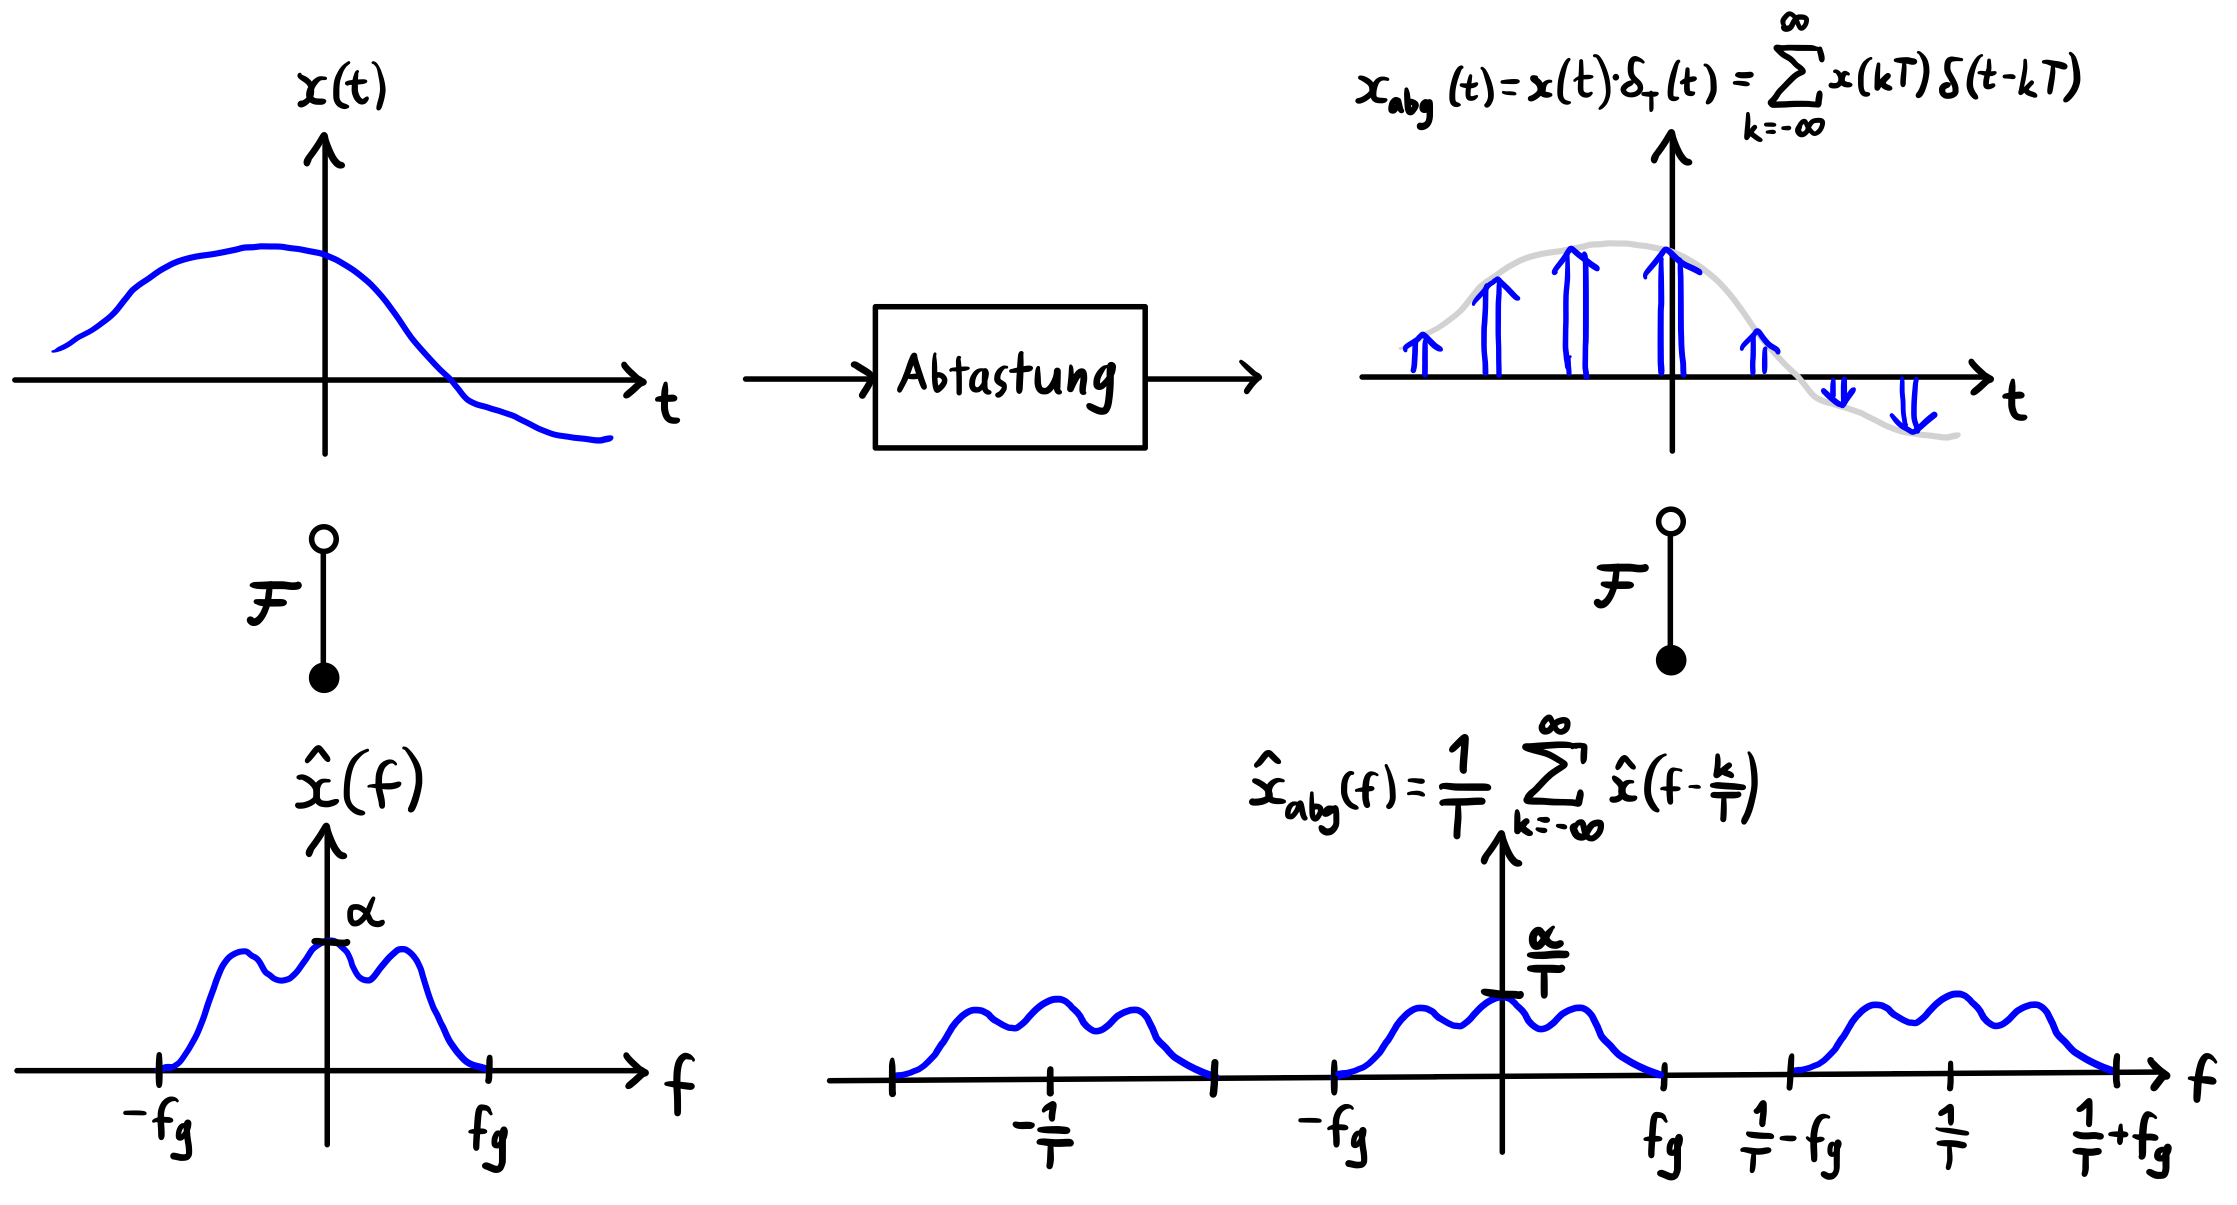
\includegraphics[width=0.92\linewidth]{figures/abtastung2.jpg}
    \end{center}
\end{frame}

\begin{frame}{Bemerkungen}
    \fcolorbox{darkblue}{lightblue}{%
    \parbox{\dimexpr\linewidth-2\fboxsep-2\fboxrule\relax}{
        \vspace{0.25cm}
        Die \textbf{Abtastung im Zeitbereich} entspricht einer \textbf{Periodisierung im Frequenzbereich}.
        \vspace{0.25cm}
    }}%
    \vspace*{12pt}
    \begin{itemize}
        \item $f_g$ ist die Bandbreite von $x(t)$
        \item[] 
        \item $f_s := \displaystyle\frac{1}{T}$ ist die Abtastfrequenz (\textit{sampling frequeny})
        \item[] 
        \item Die Kopien von $\hat{x}(f)$ sind mit Faktor $\frac{1}{T}$ skaliert.
    \end{itemize}
\end{frame}

\begin{frame}{Rekonstruktion}
    \begin{itemize}
    \item Wie gewinnen wir das analoge Signal ohne Informationsverlust aus den Abtastwerten zurück?
    \item[] \begin{center}
        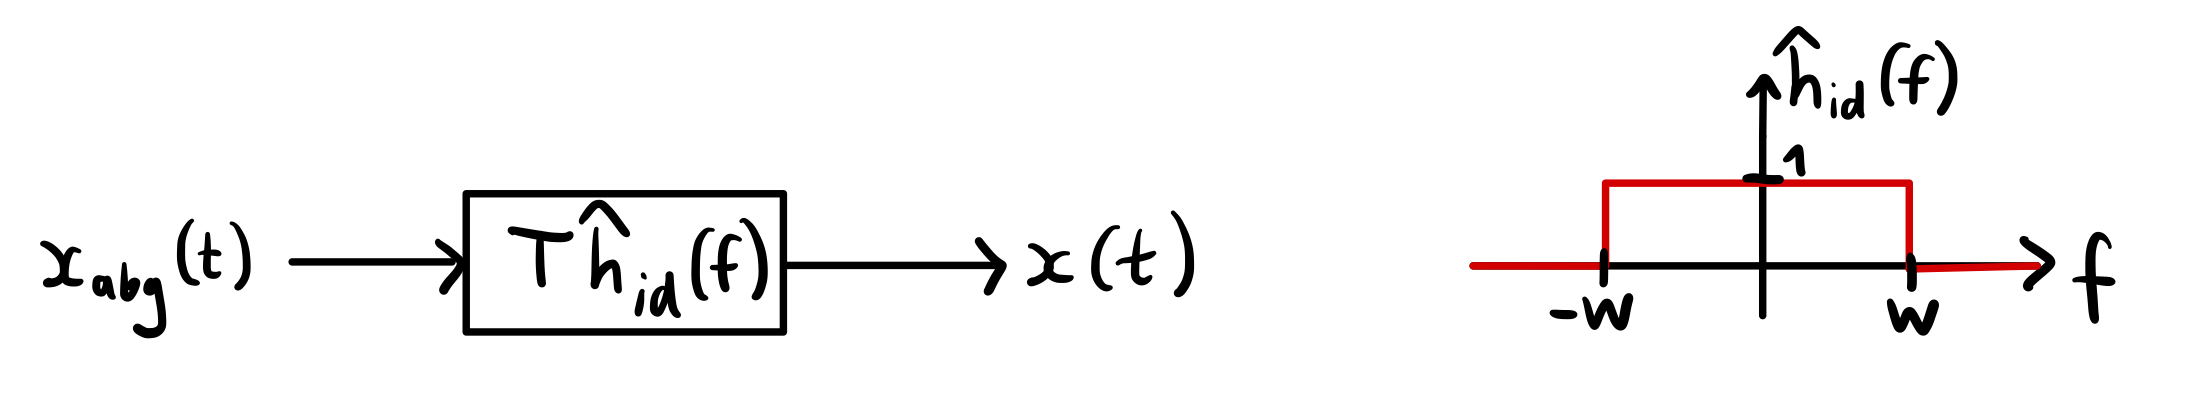
\includegraphics[width=0.75\linewidth]{figures/filtering3.jpg}
    \end{center}
    \item[] $\hat{h}_{id}(f) = \displaystyle\begin{cases}
        1, \hspace{6pt} |f|\leq W \\
        0, \hspace{6pt} |f|> W
    \end{cases}$ idealer Tiefpassfilter mit Breite $W$
    \item[] Zur Erinnerung: $\hat{x}_{abg.} = \displaystyle\frac{1}{T} \displaystyle\sum_{k = -\infty}^\infty \hat{x}\left( f- \frac{k}{T} \right)$
    \end{itemize}
\end{frame}

\begin{frame}{Rekonstruktion}
    Der Term $\cdot T$ beim idealen Tiefpassfilter steht für die Skalierung, da wir ohne diesen Term $\frac{1}{T}x(t)$ anstatt $x(t)$ erhalten würden.\\
    \begin{center}
        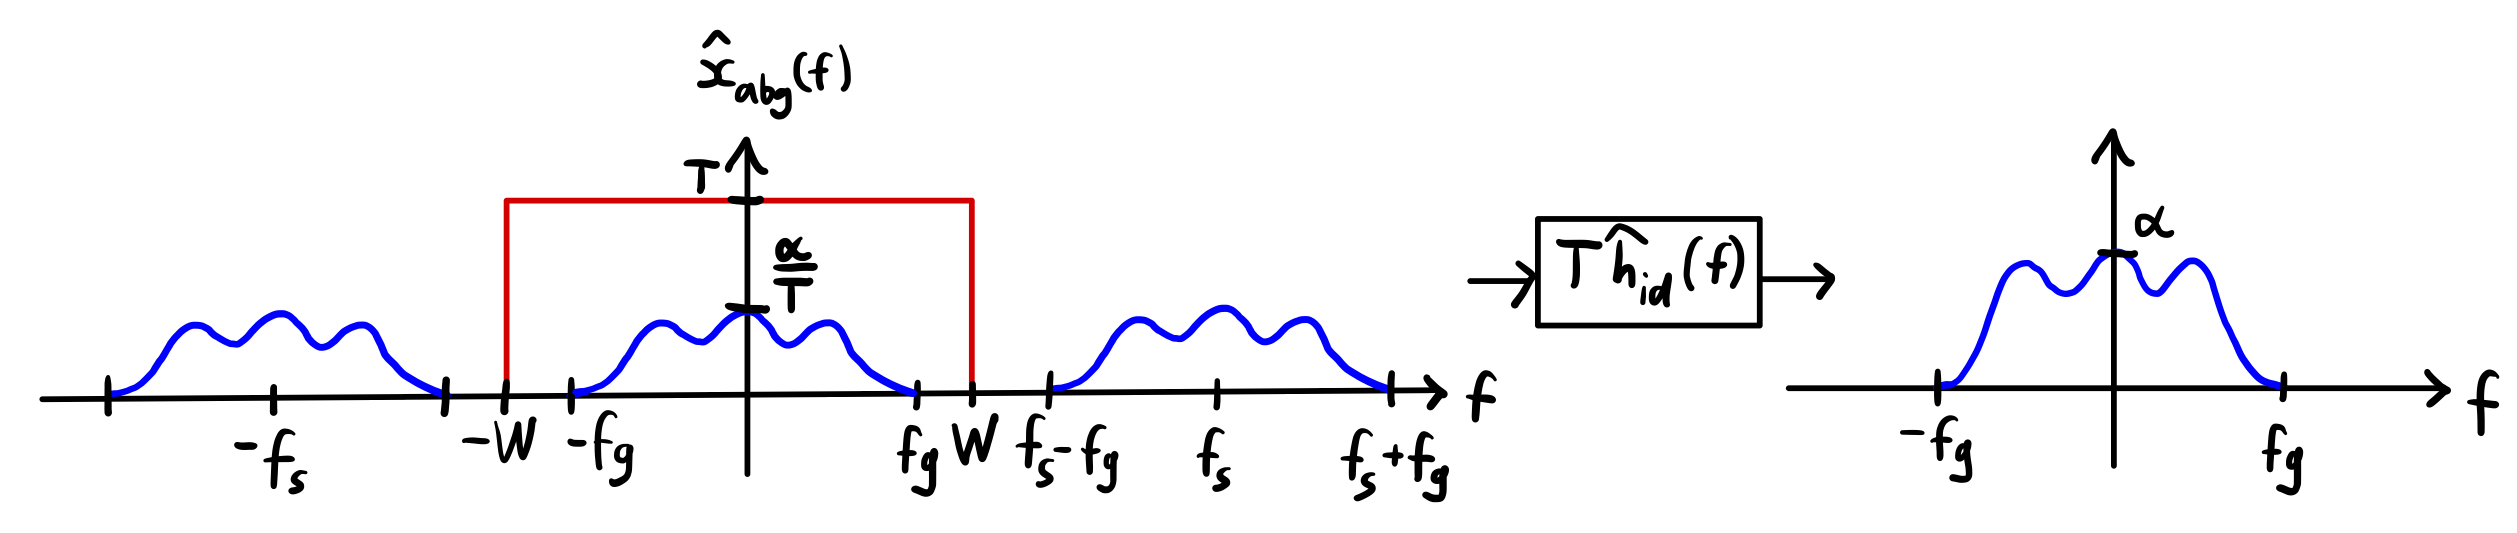
\includegraphics[width=\linewidth]{figures/filtering1.jpg}\\
    \end{center}
    \textbf{Bemerkung}: Die Wahl von $W$ ist entscheidend und in einigen Fällen ist es gar nicht möglich, das Signal zu rekonstruieren.
\end{frame}

\begin{frame}{1. \textcolor{myblue}{\textbf{Kritische Abtastung: $f_s = 2 f_g$}}}
    \begin{center}
        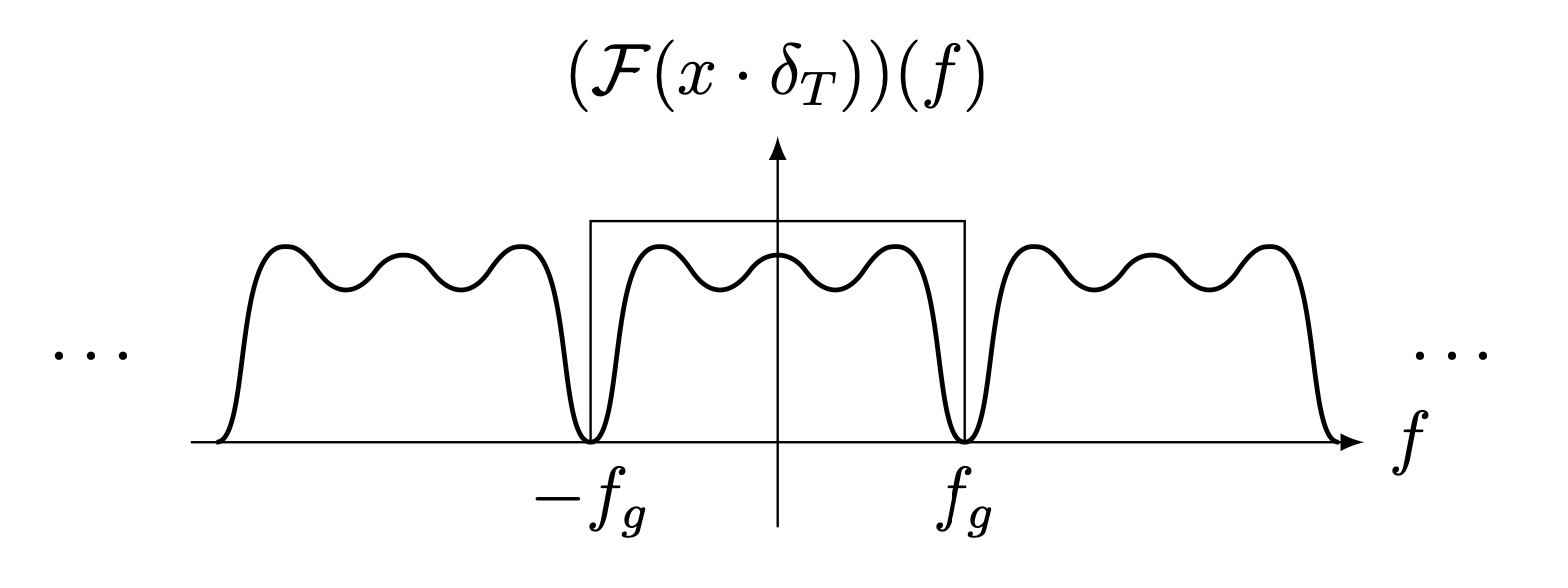
\includegraphics[width=0.85\linewidth]{figures/krit_abtast.png}
    \end{center}
    $\implies$ Wir können das Signal mit einem idealen Tiefpassfilter der Breite $W = f_g$ rekonstruieren

\end{frame}

\begin{frame}{2. \textcolor{myblue}{\textbf{Überabtastung: $f_s > 2f_g$}}}
    \begin{center}
        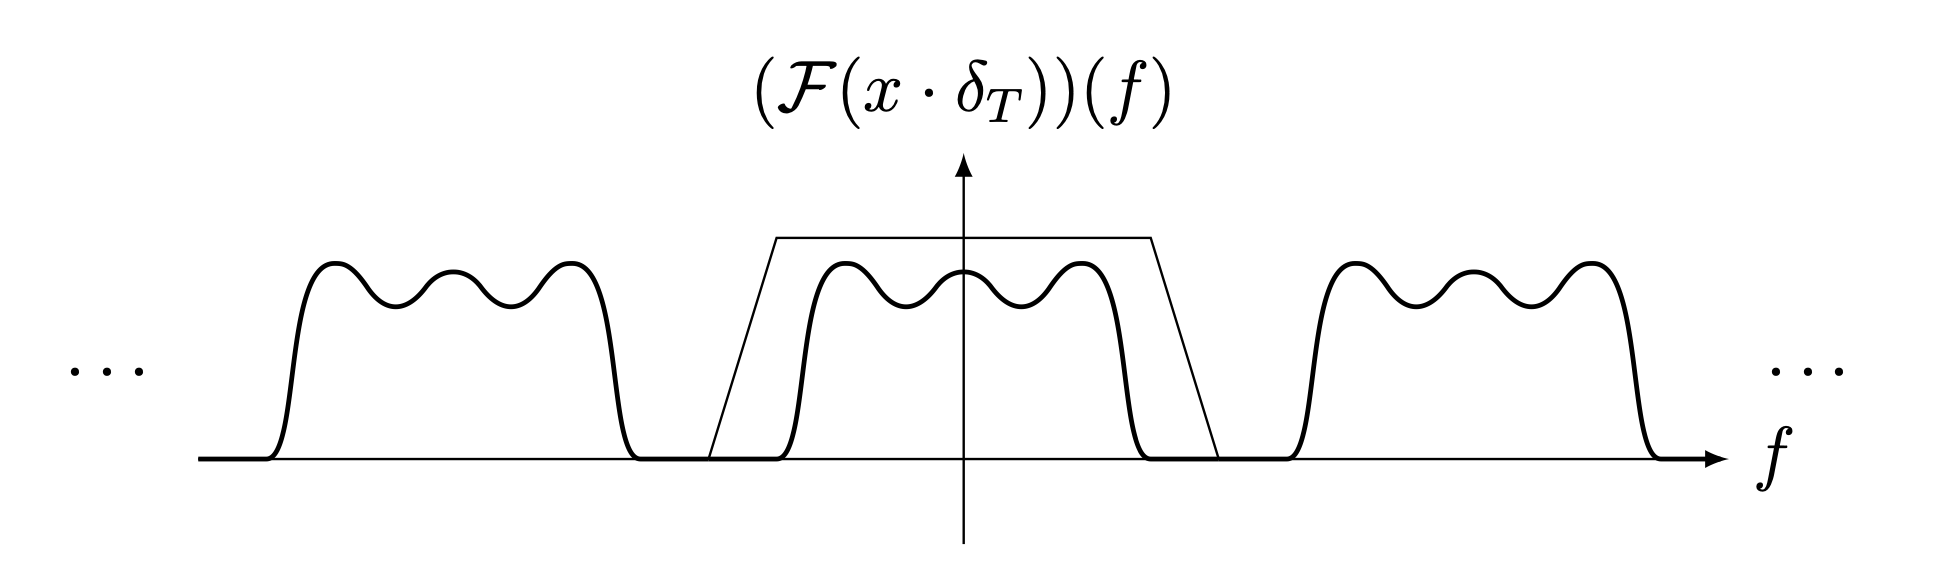
\includegraphics[width=0.85\linewidth]{figures/ueberabtast.png}
    \end{center}

\textbf{Vorteile an Überabtastung:}
\begin{enumerate}
    \item Wir können einen stabilen Tiefpassfilter verwenden.
    \item Überabtastung verringert die Empfindlichkeit auf Rauschen.
\end{enumerate}
\end{frame}

\begin{frame}{3. \textcolor{myblue}{\textbf{Unterabtastung: $f_s < 2 f_g$}}}
    \begin{center}
        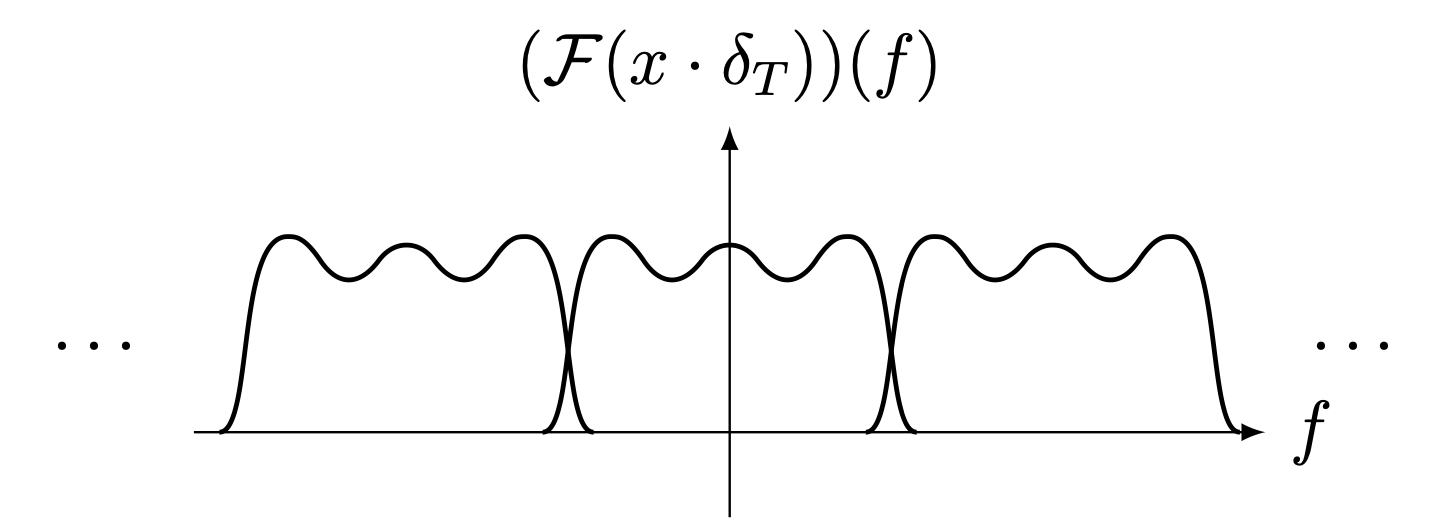
\includegraphics[width=0.8\linewidth]{figures/aliasing1.png}
    \end{center}
    Es gibt \textbf{Aliasing}. Mit Hilfe eines Tiefpassfilters erhalten wir keine perfekte Version von $\hat{x}(f)$.
\end{frame}

\begin{frame}{Intuition}
    \begin{center}
        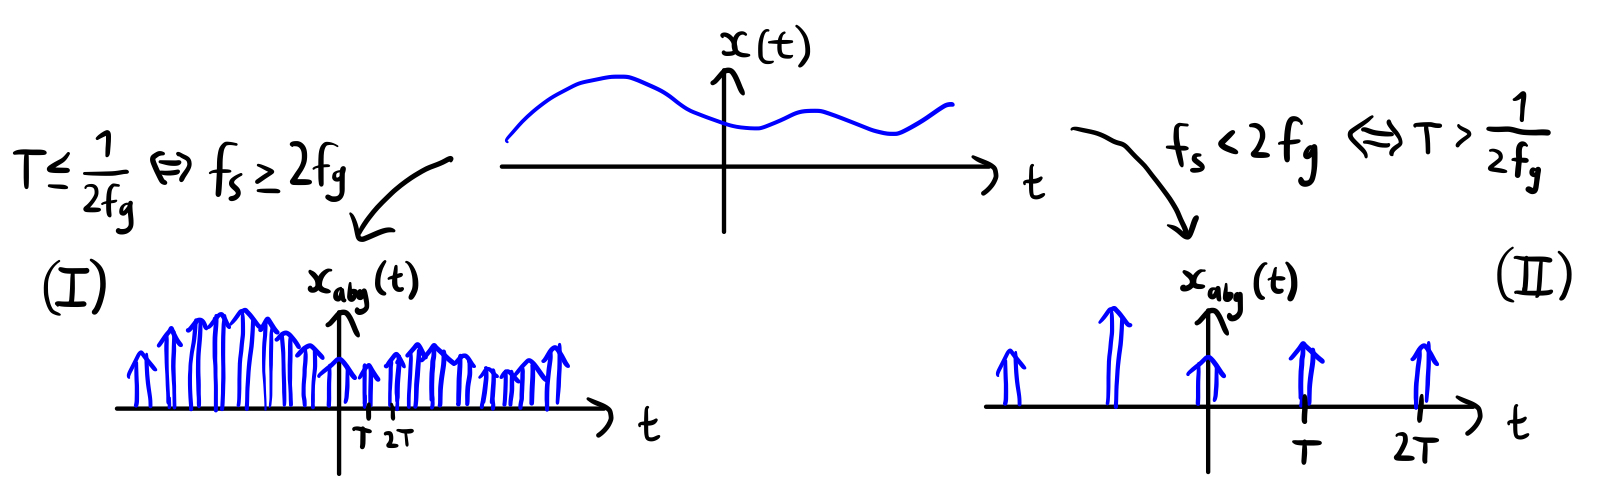
\includegraphics[width=\linewidth]{figures/aliasing2.jpg}
    \end{center}
    \begin{itemize}
        \item[(I)] Genug hohe Abtastrate $\implies$ kein Informationsverlust
        \item[(II)] Zu tiefe Abtastrate $\implies$ Informationsverlust
    \end{itemize}
\end{frame}

\begin{frame}{\textcolor{myblue}{\textbf{Abtasttheorem}}}
    \fcolorbox{darkblue}{lightblue}{%
    \parbox{\dimexpr\linewidth-2\fboxsep-2\fboxrule\relax}{
        \vspace*{0.25cm}
        Ein Signal mit der Bandbreite $f_g$ kann aus seinen Abtastwerten, genommen mit einer Rate von $f_s \geq 2f_g$, eindeutig rekonstruiert werden.\\
        Die kritische Rate $f_s = 2 f_g$ wird als \textbf{Nyquistrate} bezeichnet.
        \vspace*{0.25cm}
    }}%
\end{frame}

\begin{frame}{Interpretation als Interpolation}
    \begin{itemize}
    \item Wir betrachten das folgende System:
    \item[] 
    \item[] \begin{center}
        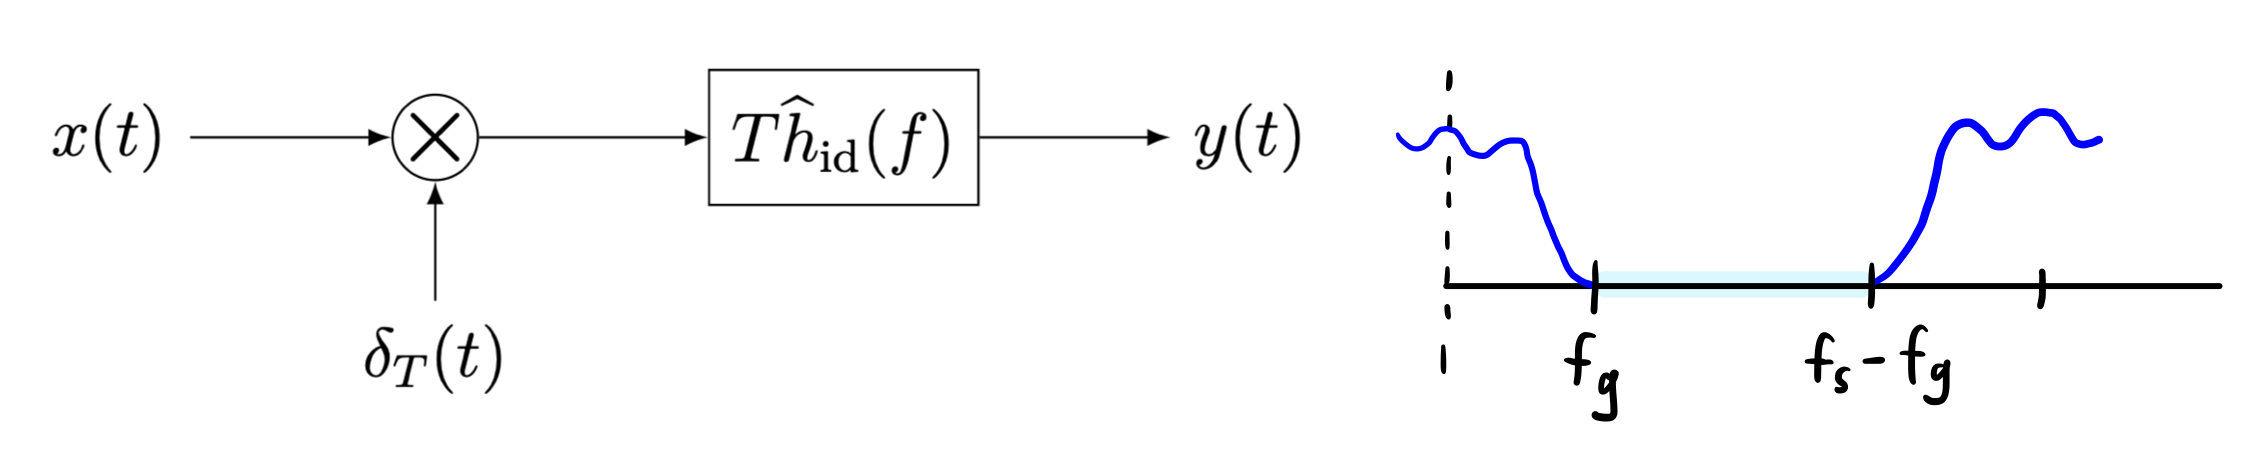
\includegraphics[width=0.9\linewidth]{figures/filtering2.jpg}
    \end{center}
    \item[] 
    \item[] wobei $\hat{h}_{id}(f) = \displaystyle\begin{cases}
        1, \; |f| \leq W \\
        0, \; |f| > W
    \end{cases} \invtransform{}{1} \; h_{id}(t)=\displaystyle\frac{\sin(2 \pi W t)}{\pi t}$
    \item[] 
    \item Damit die perfekte Rekonstruktion möglich ist, muss $W \in [f_g, \; f_s -f_g]$ und $f_s \geq 2f_g$ gelten.
    \end{itemize}
\end{frame}

\begin{frame}{Interpretation als Interpolation}
    \vspace*{-0.5cm}
    \begin{align*}
        y(t) &= \left(\underbrace{(x \cdot \delta_T)}_{x_{abg}} \ast T h_{id}\right)(t) = T (x_{abg} \ast h_{id})(t) \\
        &= T \left[ \left( \sum_{k = -\infty}^{\infty} x(kT) \delta(\cdot -kT) \right)  \ast h_{id} \right](t) \\
        &= T \left( \sum_{k = -\infty}^{\infty} x(kT) \left(\delta(\cdot -kT) \right)  \ast h_{id}\right) (t) \\
        &= T \sum_{k = -\infty}^{\infty} x(kT) h_{id}(t-kT)
    \end{align*}
\end{frame}

\begin{frame}{Rekonstruktionsformel}
    \begin{itemize}
        \item[] Also: $y(t) = T \displaystyle\sum_{k = -\infty}^{\infty} x(kT) h_{id}(t-kT), \hspace{12pt} \text{wobei}$
        \item[] $h_{id} = \displaystyle\frac{\sin(2 \pi W t)}{\pi t}$
        \item[] 
        \item[]  Somit erhalten wir die \textbf{Rekonstruktionsformel}:
        \item[] 
    \end{itemize}
    \fcolorbox{darkblue}{lightblue}{%
    \parbox{\dimexpr\linewidth-2\fboxsep-2\fboxrule\relax}{
        $$y(t) = T \sum_{k = -\infty}^\infty x(kT) \frac{\sin\left( 2 \pi W (t-kT)\right)}{\pi (t-kT)}$$
    }}%
\end{frame}

\begin{frame}{Kritische Abtastung}
    \begin{itemize}
    \item Kritische Abtastung: $f_s = 2 f_g$, d.h. $f_g = f_s - f_g$
    \item[] $\implies W = f_g = \frac{f_s}{2} = \frac{1}{2T}$
    \item[] $\implies y(t) = x(t) = \displaystyle\sum_{k=-\infty}^\infty x(kT)\displaystyle\frac{\sin\left(\frac{\pi}{T}(t-kT)\right)}{\frac{\pi}{T}(t-kT)}$
    \item[] 
    \item Allgemeine Rekonstruktion eines Signals aus Abtastwerten:
    \item[] 
    \fcolorbox{darkblue}{lightblue}{%
    \parbox{\dimexpr\linewidth-2\fboxsep-2\fboxrule\relax}{
       $$y(t) = T \displaystyle\sum_{k = -\infty}^\infty x(kT)h(t-kT)$$
    }}%
    \item[] 
    \item $h(t)$ ist die Impulsantwort eines Filters.
\end{itemize}
\end{frame}

\begin{frame}{Abtastung als Entwicklung in ein Orthonormalsystem}
    Die Rekonstruktionsformel
    $$x(t) = \sum_{k=-\infty}^\infty x(kT)\displaystyle\frac{\sin\left(\frac{\pi}{T}(t-kT)\right)}{\frac{\pi}{T}(t-kT)}$$
    entspricht einer Entwicklung eines bandbegrenzten Signals $x(t)$ in ein Orthonormalsystem.
\end{frame}

\begin{frame}{Abtastung als Entwicklung in ein Orthonormalsystem}
    Linearer Unterraum $X$ der $f_g-$bandbegrenzten Signale in $L^2(\mathbb{R})$
    $$e_k(t) = \frac{1}{\sqrt{T}}\frac{\sin\left(\frac{\pi}{T}(t-kT)\right)}{\frac{\pi}{T}(t-kT)} = \sqrt{T} \frac{\sin\left(\frac{\pi}{T}(t-kT)\right)}{\pi(t-kT)}$$
    Diese Funktionen bilden ein Orthonormalsystem in $X$. Es gilt:
    $$x(t) = \sum_{k=-\infty}^\infty \sqrt{T}x(kT)\underbrace{\frac{1}{\sqrt{T}}\frac{\sin\left(\frac{\pi}{T}(t-kT)\right)}{\frac{\pi}{T}(t-kT)}}_{e_k} = \sum_{k = -\infty}^\infty \langle x, \; e_k \rangle \cdot e_k$$
\end{frame}

\begin{frame}{Prüfungsaufgabe: Frühjahr 2023, Aufgabe 2}
    
\end{frame}

\end{document}
